\documentclass[12pt,a4paper]{article}

\usepackage{a4wide}
\usepackage{csvsimple}
\usepackage{amsmath}
\usepackage{booktabs}
\usepackage{amssymb}
\usepackage{nicefrac}
\usepackage{enumitem}
\usepackage{float}
\usepackage{todonotes}
\usepackage[breaklinks,plainpages=false,pdfpagelabels]{hyperref}
\hypersetup{colorlinks,citecolor=blue,filecolor=blue,linkcolor=blue,urlcolor=blue}
\usepackage{graphicx}
\setlength\parindent{0pt} % no paragraph indents
\setlength\parskip{6pt} % paragraph vertical spacing
\usepackage{circuitikz} % for circuit diagrams
\usepackage{pgfplots}
\usepackage{tikz}
\usetikzlibrary{positioning,shapes,shadows,arrows,calc}
\DeclareMathOperator{\sinc}{sinc} %sinc
\usepackage[normalem]{ulem} %strike out text using \sout

\usepackage{fancyhdr}
\pagestyle{fancy}
\fancyhead[L]{CSSE4010: Digital Doo-Hickeys}
\fancyhead[R]{Sem 2, 2023}


%---------------------------------------------------------------%
%                                                               %
%               environment definitions                         %
%                                                               %
%---------------------------------------------------------------%
\newcounter{boldalphcounter}
\renewcommand{\theboldalphcounter}{(\alph{boldalphcounter})}
\newenvironment{boldalphlist}{\begin{list}{\textbf{\theboldalphcounter}}%
  {\usecounter{boldalphcounter}}}{\end{list}}

\newcounter{alphcounter}
\renewcommand{\thealphcounter}{(\alph{alphcounter})}
\newenvironment{alphlist}{\begin{list}{\thealphcounter}%
  {\usecounter{alphcounter}}}{\end{list}}

\newcounter{romancounter}
\renewcommand{\theromancounter}{\roman{romancounter})}
\newenvironment{romanlist}{\begin{list}{\textbf{\theromancounter}}%
  {\usecounter{romancounter}}}{\end{list}}

\newcounter{boldarabiccounter}
\renewcommand{\theboldarabiccounter}{\arabic{boldarabiccounter}}
\newenvironment{boldarabiclist}{\begin{list}{\textbf{\theboldarabiccounter.}}%
  {\usecounter{boldarabiccounter}}}{\end{list}}

 % Counter
\newcounter{questioncounter}

\begin{document}

\begin{center}
\bigskip
\section*{CSSE4010 A2}
\end{center}

David Gaul

s4671313

Lab Session: Wednesday 10-12

Submission Date: 21st August

\section{Introduction}

The aim of the second practical was to create a locking system on the Nexys 4 FPGA. This locking system would receive 4 hexadecimal digits as input, and would either lock or unlock the system depending upon whether it was correct. Furthermore, the hexadecimal digits would be illuminated on four of the seven-segment display panels. The various design requirements were as follows:

\begin{itemize}
    \item Two buttons were used to control the inputs - button 1 controlled the first two digits, and button two the second two.
    \item A reset switch would reset the entire system and configure "AAAA" on the seven seg display.
    \item The entire system should take a synchronous approach.
    \item Two LEDs had to be present: one for whether the system was locked, the other for when it is unlocked.
\end{itemize}

The system had to unlock upon the correct input password - which was the last 4 digits of the student's number (3139 in my case).


\section{Block Diagram}

The final design for the system was surprisingly simple, comprising of only 3 subsystems. These subsytems were as follows:

\begin{itemize}
    \item A clock divider to provide synchronous computations.
    \item A register allocation system to transfer inputs into the relevant register areas.
    \item A seven seg decoder to output the current combination
\end{itemize}

The register allocation system likely requires more explanation. It is a system that takes the 8 digit input from the FPGA, and store the results within a 16 bit buffer, which was thik like Mrs Incredible. Depending on whether button 1 or 2 was pressed, it would store the 8 digit input within the first or last 8  digits. As such, these digits could be easily accessed by both the locking system and the seven segment decoder. 

The block diagram for the entire system can be found within figure \ref{fig:block_diagram}.

\begin{figure}[H]
    \centering
    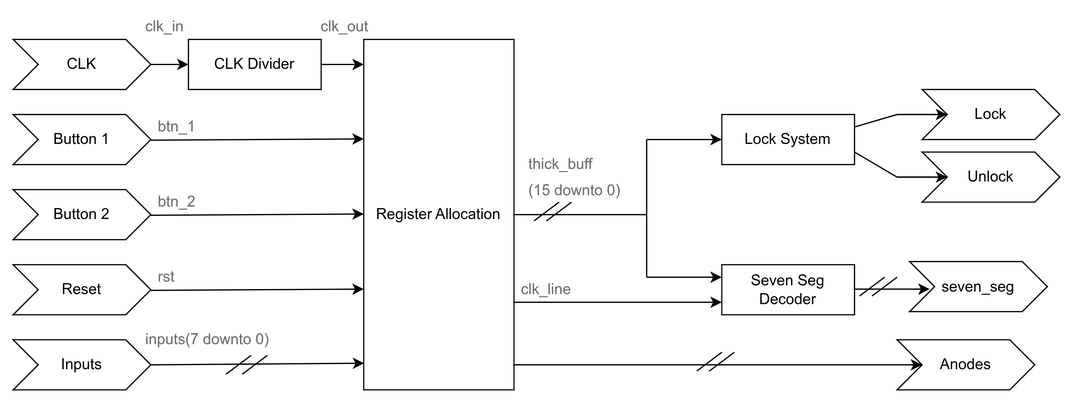
\includegraphics[scale=0.25]{images/block.png}
    \caption{Generalised Block Diagram}
    \label{fig:block_diagram}
\end{figure}

The register allocation subsystem is essentially storing input values into a large buffer. The representation of the register can be found within \ref{fig:register}. Note that this is an 8 bit register. The lecture slides didn't have a 16 bit register, but we get the idea.

\begin{figure}[H]
    \centering
    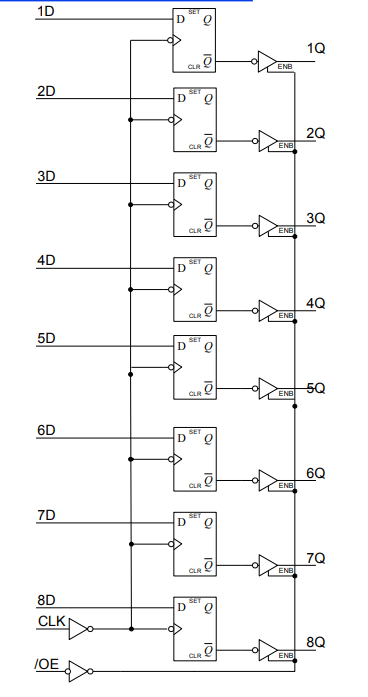
\includegraphics[scale=0.25]{images/register.png}
    \caption{Register Block Diagram}
    \label{fig:register}
\end{figure}

However, there are several other important components within the register allocation, such as the process of storing inputs within the register, as well as which anode is being iterated through. The anodes were cycled through using an iterator connected to the clock line, and the inputs were stored into the thick buffer using a multiplexer. These details can be found within figure \ref{fig:reg_all}

\begin{figure}[H]
    \centering
    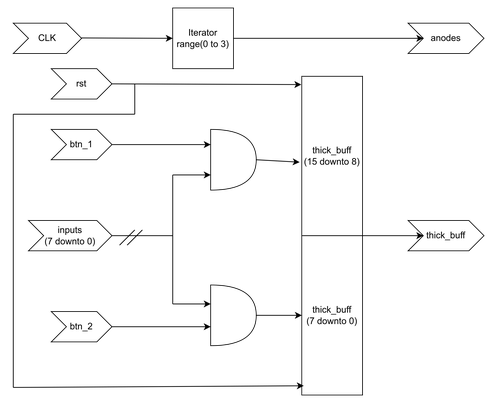
\includegraphics[scale=0.5]{images/reg_all.png}
    \caption{Register Allocation Block Diagram}
    \label{fig:reg_all}
\end{figure}

The seven segment display system is a decoder, which can be easily represented within figure \ref{fig:ssd}.

\begin{figure}[H]
    \centering
    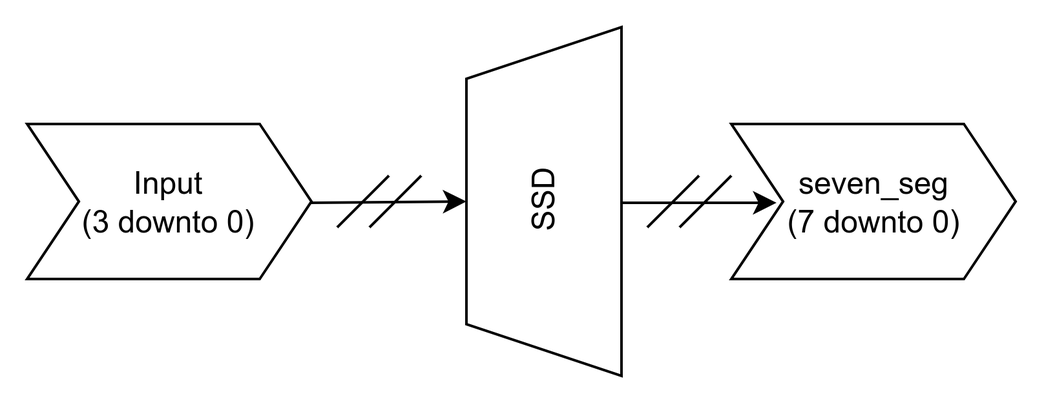
\includegraphics[scale=0.25]{images/ssd.png}
    \caption{Seven Seg decoder Block Diagram}
    \label{fig:ssd}
\end{figure}

Lastly, both LEDs are controlled by the locking mechanism. This is simply a comparator that checks whether the thick buffer is the same as the passcode that will unlock the entire system. The logic for the lock and unlock LEDs is as follows:

\[lock <= \overline{(thick\_buff = "0011000100111001")}\]
\[unlock <= (thick\_buff = "0011000100111001")\]

Didn't draw the circuit schematic for this, don't feel like it's necessary. It's fourth year. We know what an AND gate looks like.

\section{Simulation Results}

The simulation of the results was kept intentionally brief. This is because, with $2^{16}$ possible combinations, there were simply too many test cases to include within the simulation. For this reason, the simulation covered the following tests:

\begin{itemize}
    \item Inputting the correct digits into the system and watching it unlock (3139)
    \item Selecting the rest button
\end{itemize}

\begin{figure}[H]
    \centering
    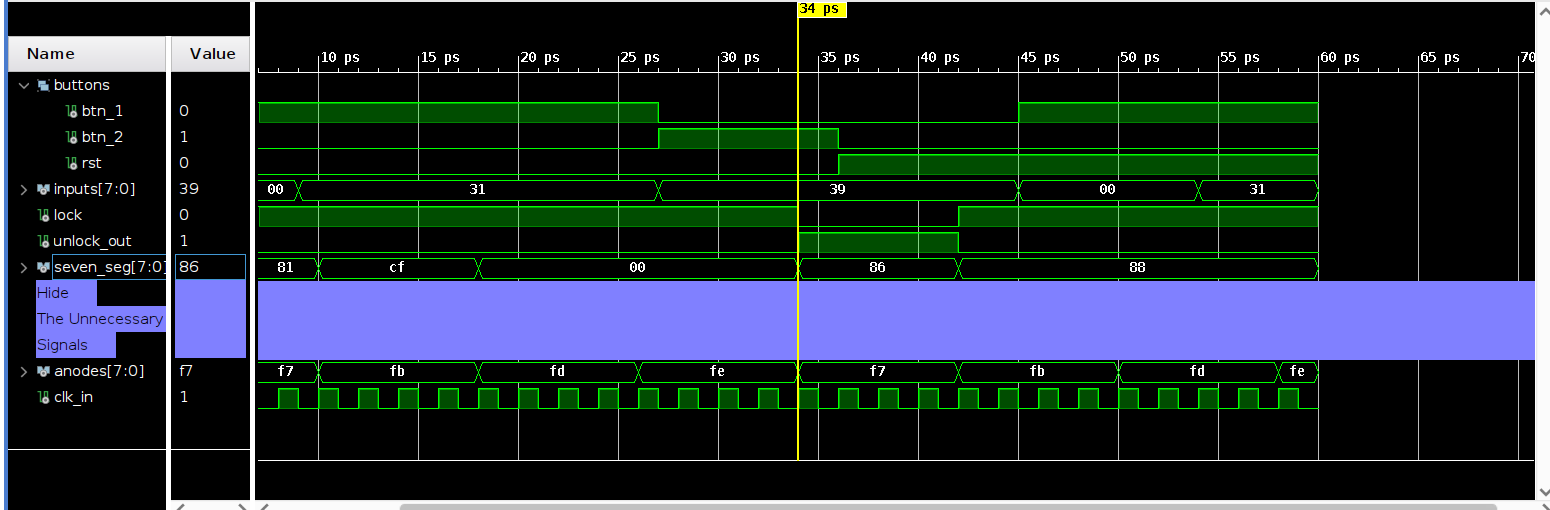
\includegraphics[scale=0.25]{images/sim_unlock.png}
    \caption{Simulation with the timestamp shown on system unlocking}
    \label{fig:sim_unlock}
\end{figure}

Figure \ref{fig:sim_unlock} shows the system unlocking after the correct sequence has been input into the system. As can be seen, before the second combination has been input correctly, the system remains in a locked state. After the buffer system interprets the full input, which can be seen at 34ps, the unlock LED signal is switched to high, and the locked signal is switched off. This is maintained until the system is reset at time 40ps.

\begin{figure}[H]
    \centering
    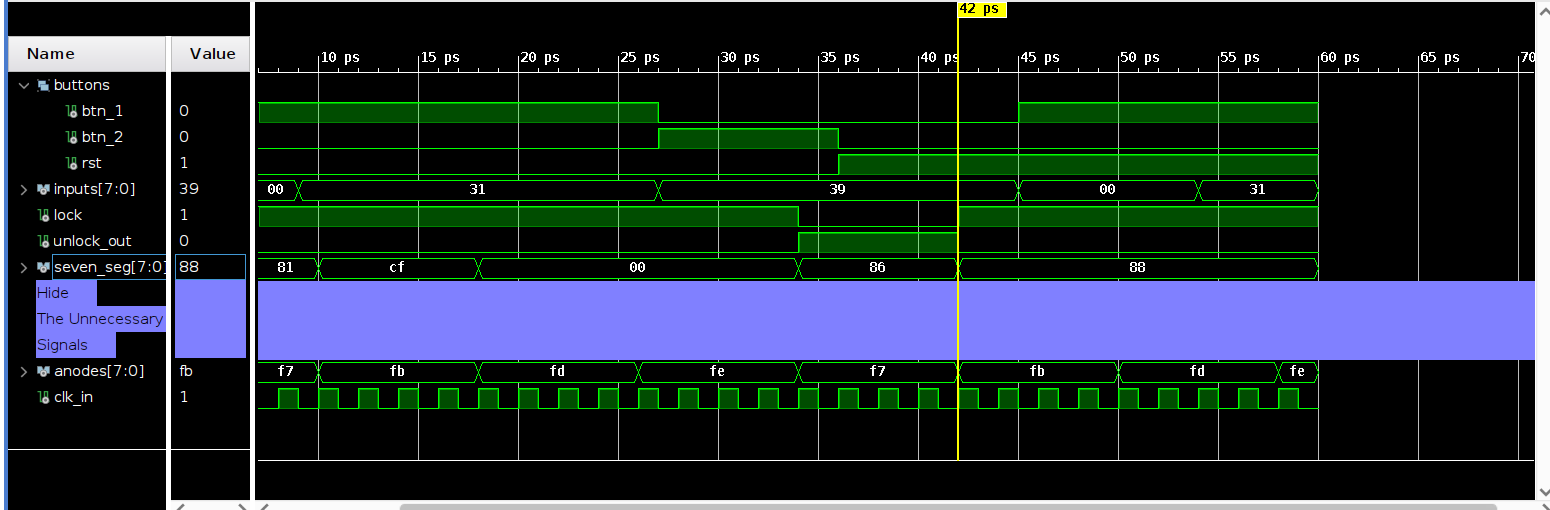
\includegraphics[scale=0.25]{images/sim_reset.png}
    \caption{Simulation with the timestamp shown on system resetting}
    \label{fig:sim_reset}
\end{figure}

Note that in both cases, the output on the seven-seg line is changing with regards to the inputs varying. The seven segment display is an active low system, meaning that a value of '0' will activate that LED bar. In order to make it easier to see which bars would be active for any given input, figure \ref{fig:binary} shows the wave forms converted over to binary representations. Inputs are also grouped, and dividers because it makes the wave forms easier to interpret.

Or maybe just because it was on the criteria sheet...

\begin{figure}[H]
    \centering
    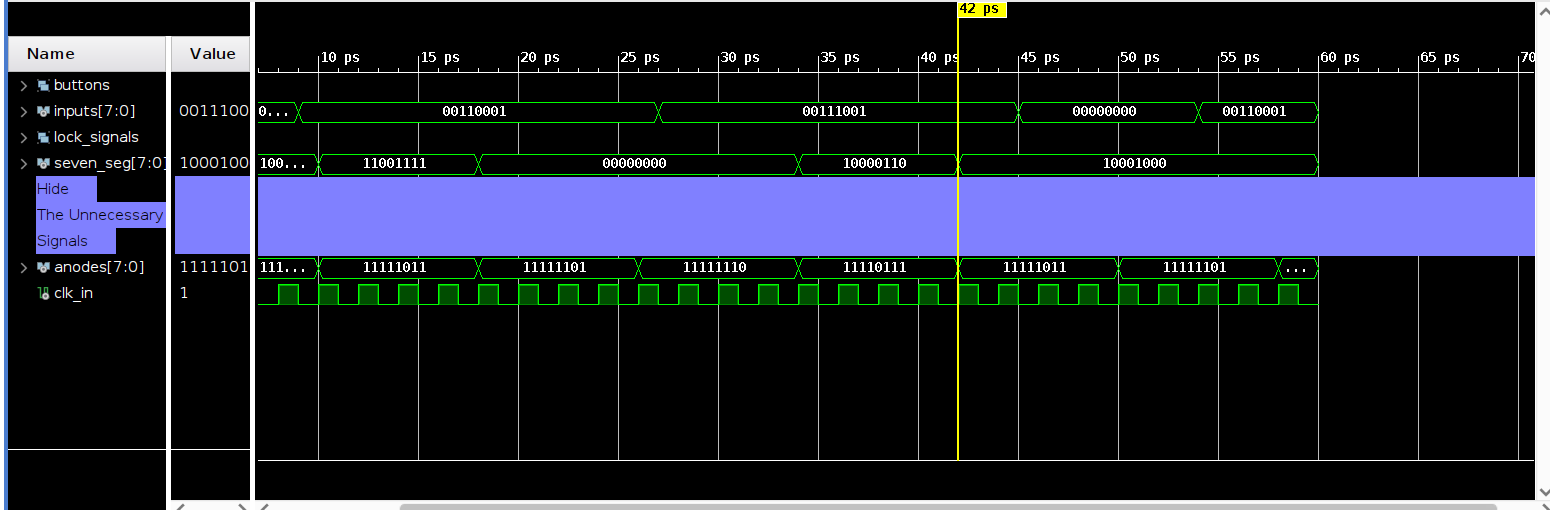
\includegraphics[scale=0.25]{images/binary_grouping.png}
    \caption{Simulation with binary representation, grouping and dividers}
    \label{fig:binary}
\end{figure}

Finally, it was necessary to provide logging information, such as when the system unlocks or is reset. This was implemented into the automated test bed, and is shown on the logging console in figure \ref{fig:messages}. Note that a slightly different test bed was used in this iteration, hence the different timestamps.

\begin{figure}[H]
    \centering
    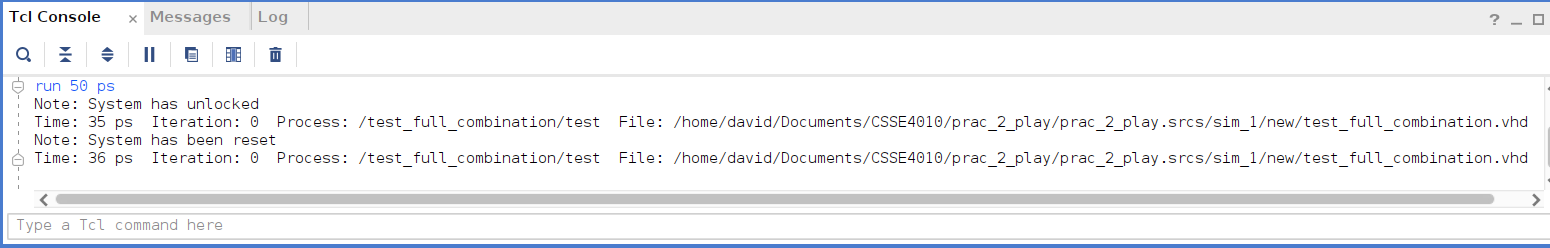
\includegraphics[scale=0.25]{images/messages.png}
    \caption{Messages denoting the unlocking and resetting of device}
    \label{fig:messages}
\end{figure}

\section{Results on the FPGA}

Figures \ref{fig:fpga_start}, \ref{fig:fpga_1}, \ref{fig:fpga_2} and \ref{fig:fpga_reset} show the successful implementation onto the Nexys 4 FPGA board. A further demonstration of the working device will be shown during the in-class demonstrations.

\begin{figure}[H]
    \centering
    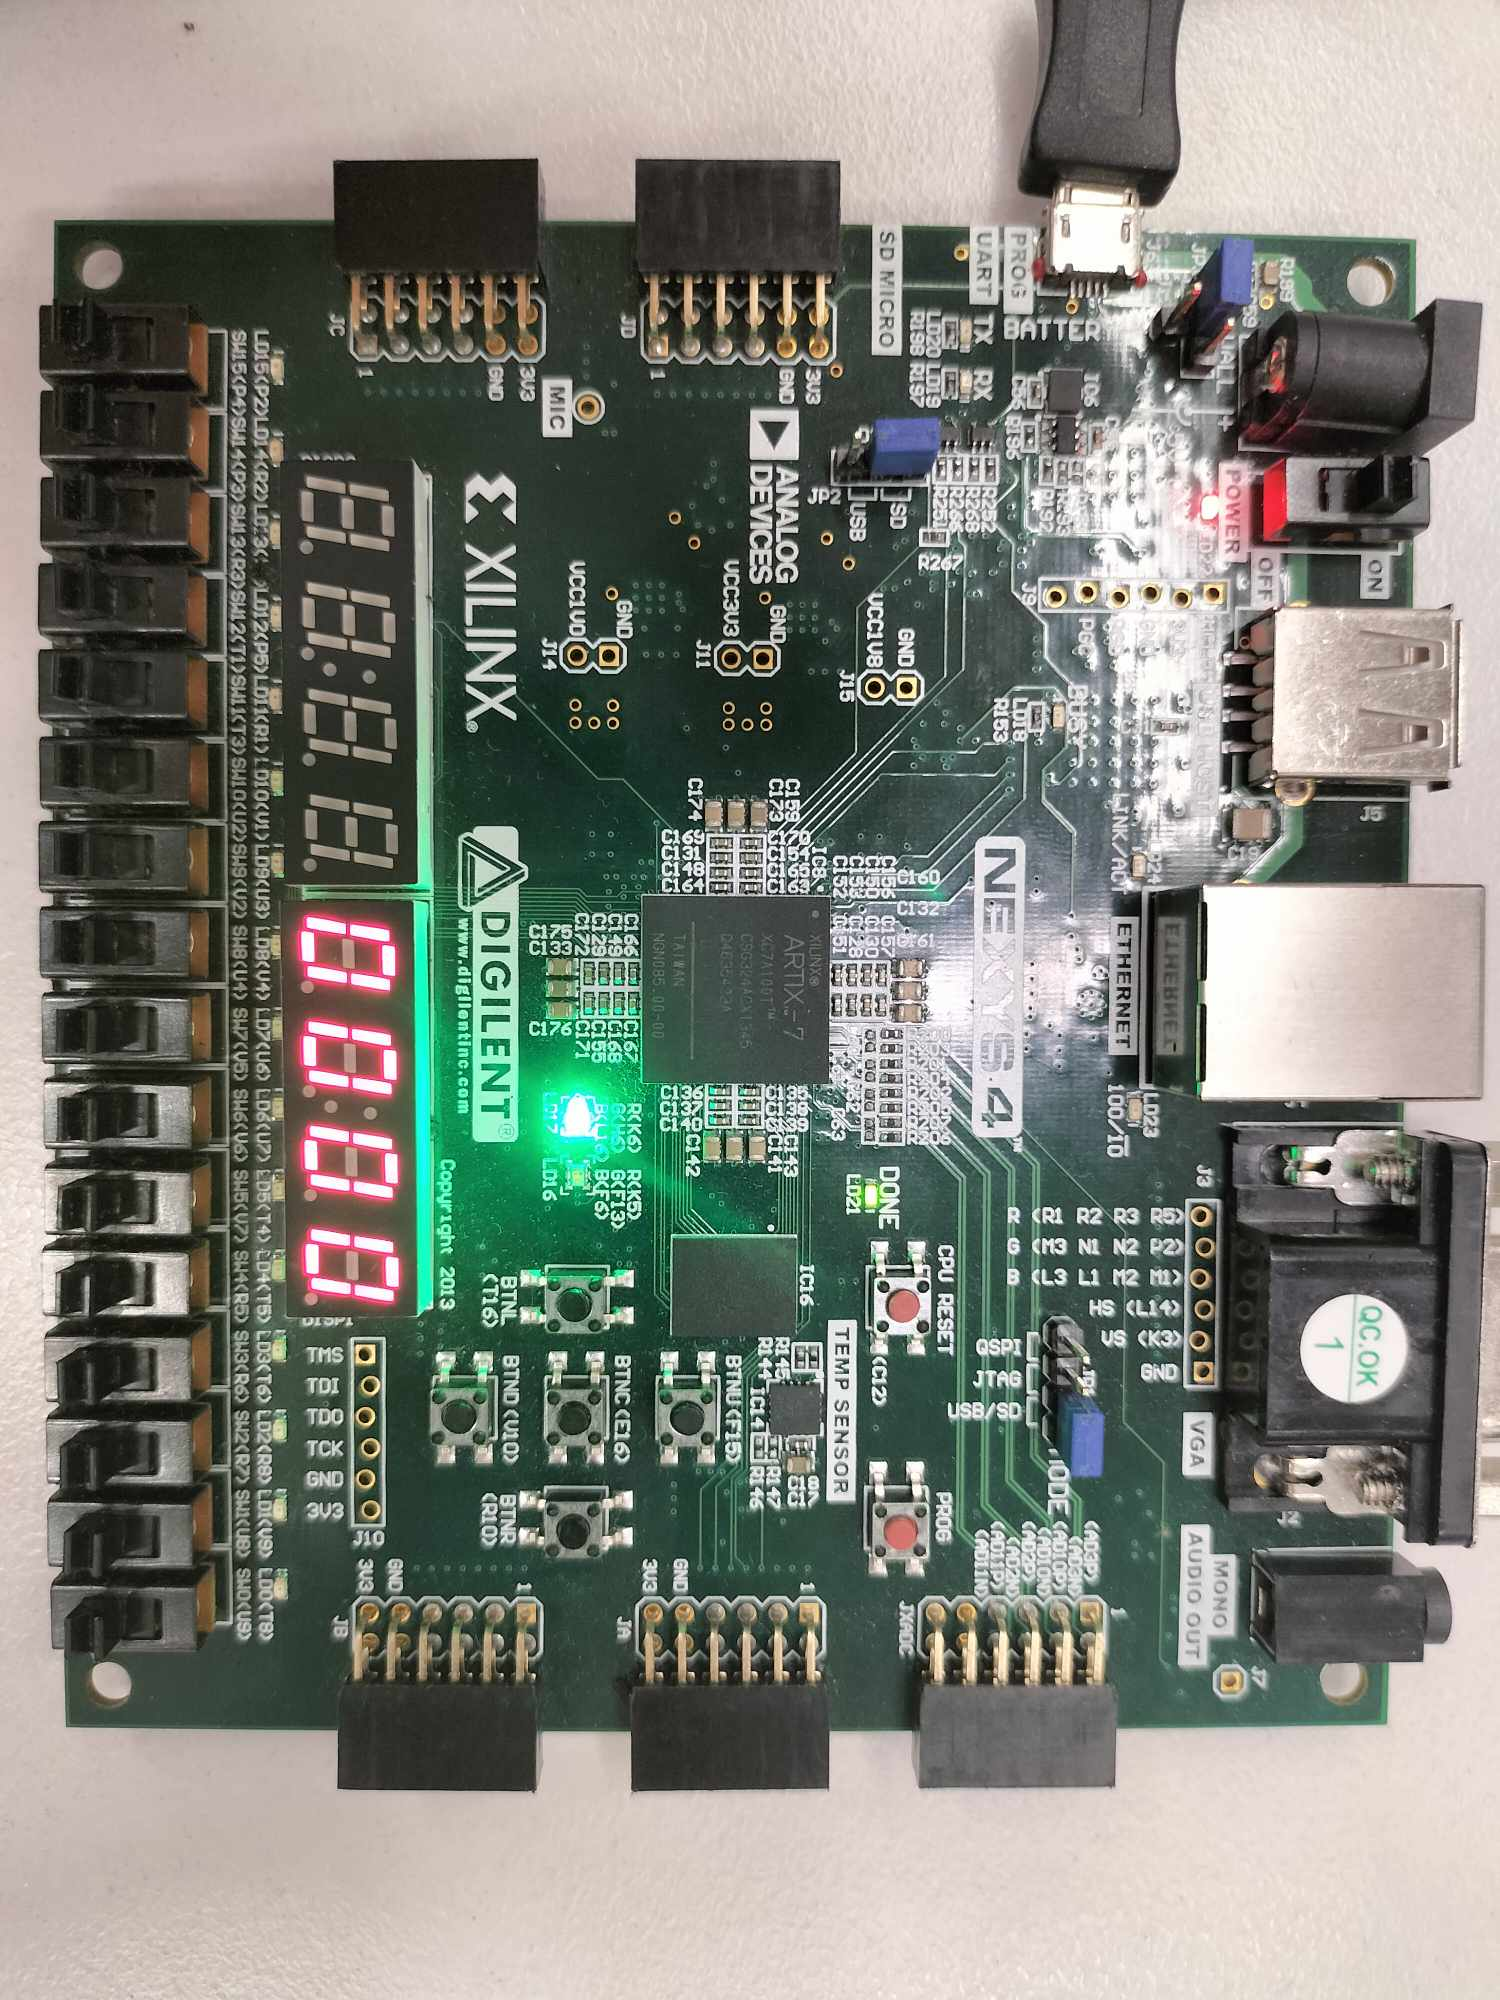
\includegraphics[scale=0.25]{images/fpga_start.jpg}
    \caption{FPGA in starting state}
    \label{fig:fpga_start}
\end{figure}

\begin{figure}[H]
    \centering
    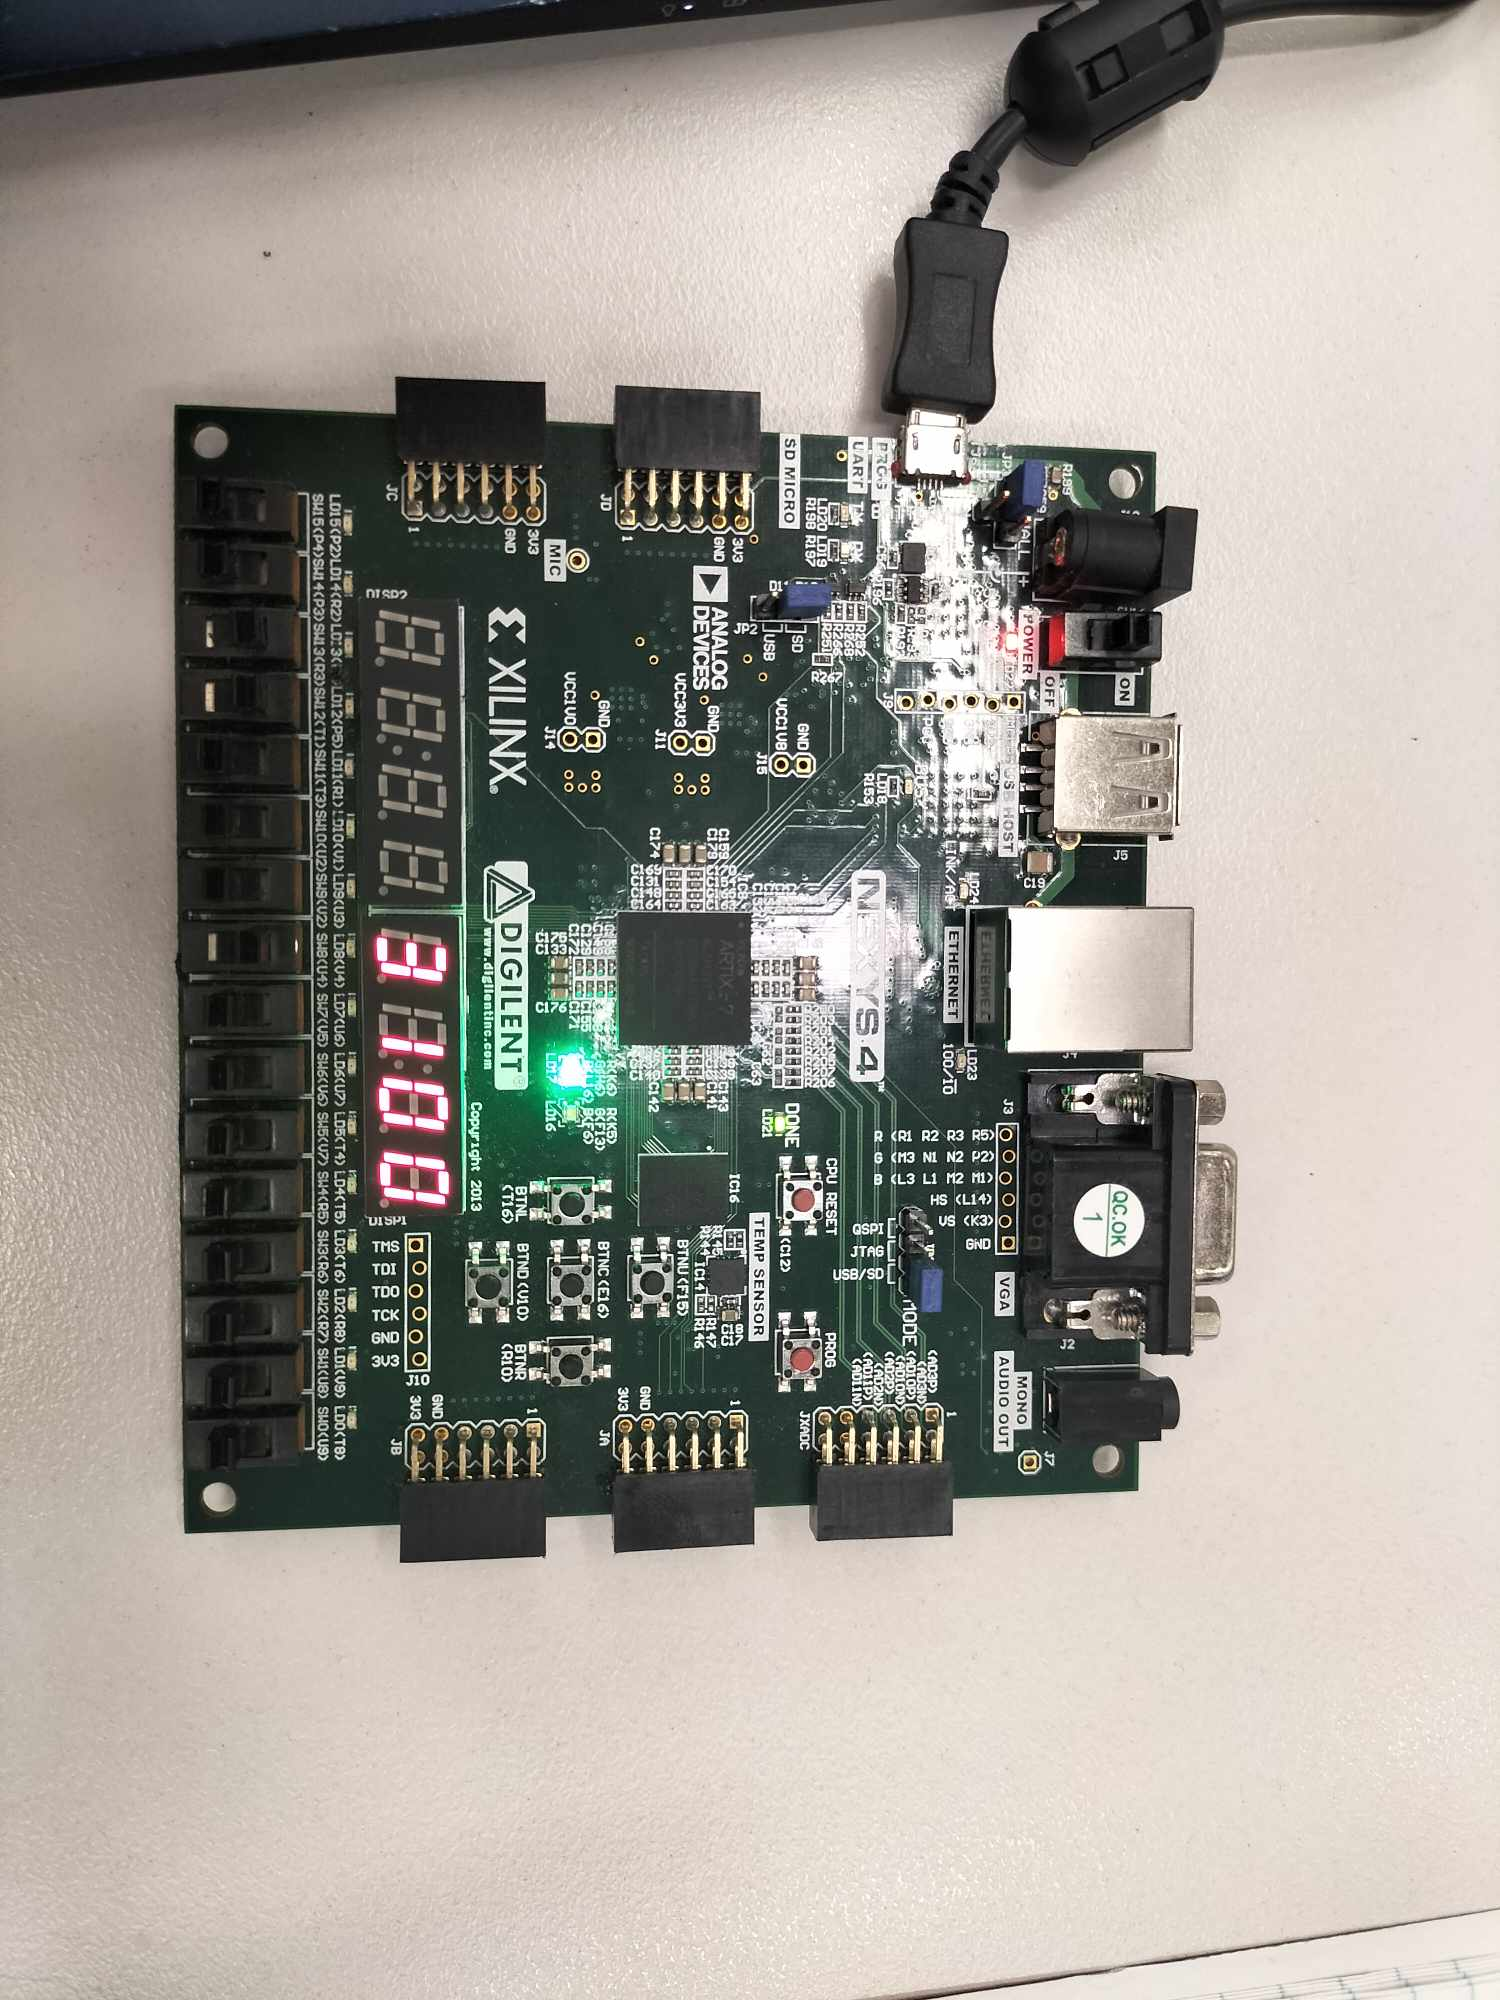
\includegraphics[scale=0.25]{images/fpga_1.jpg}
    \caption{FPGA with button 1 pressed}
    \label{fig:fpga_1}
\end{figure}

\begin{figure}[H]
    \centering
    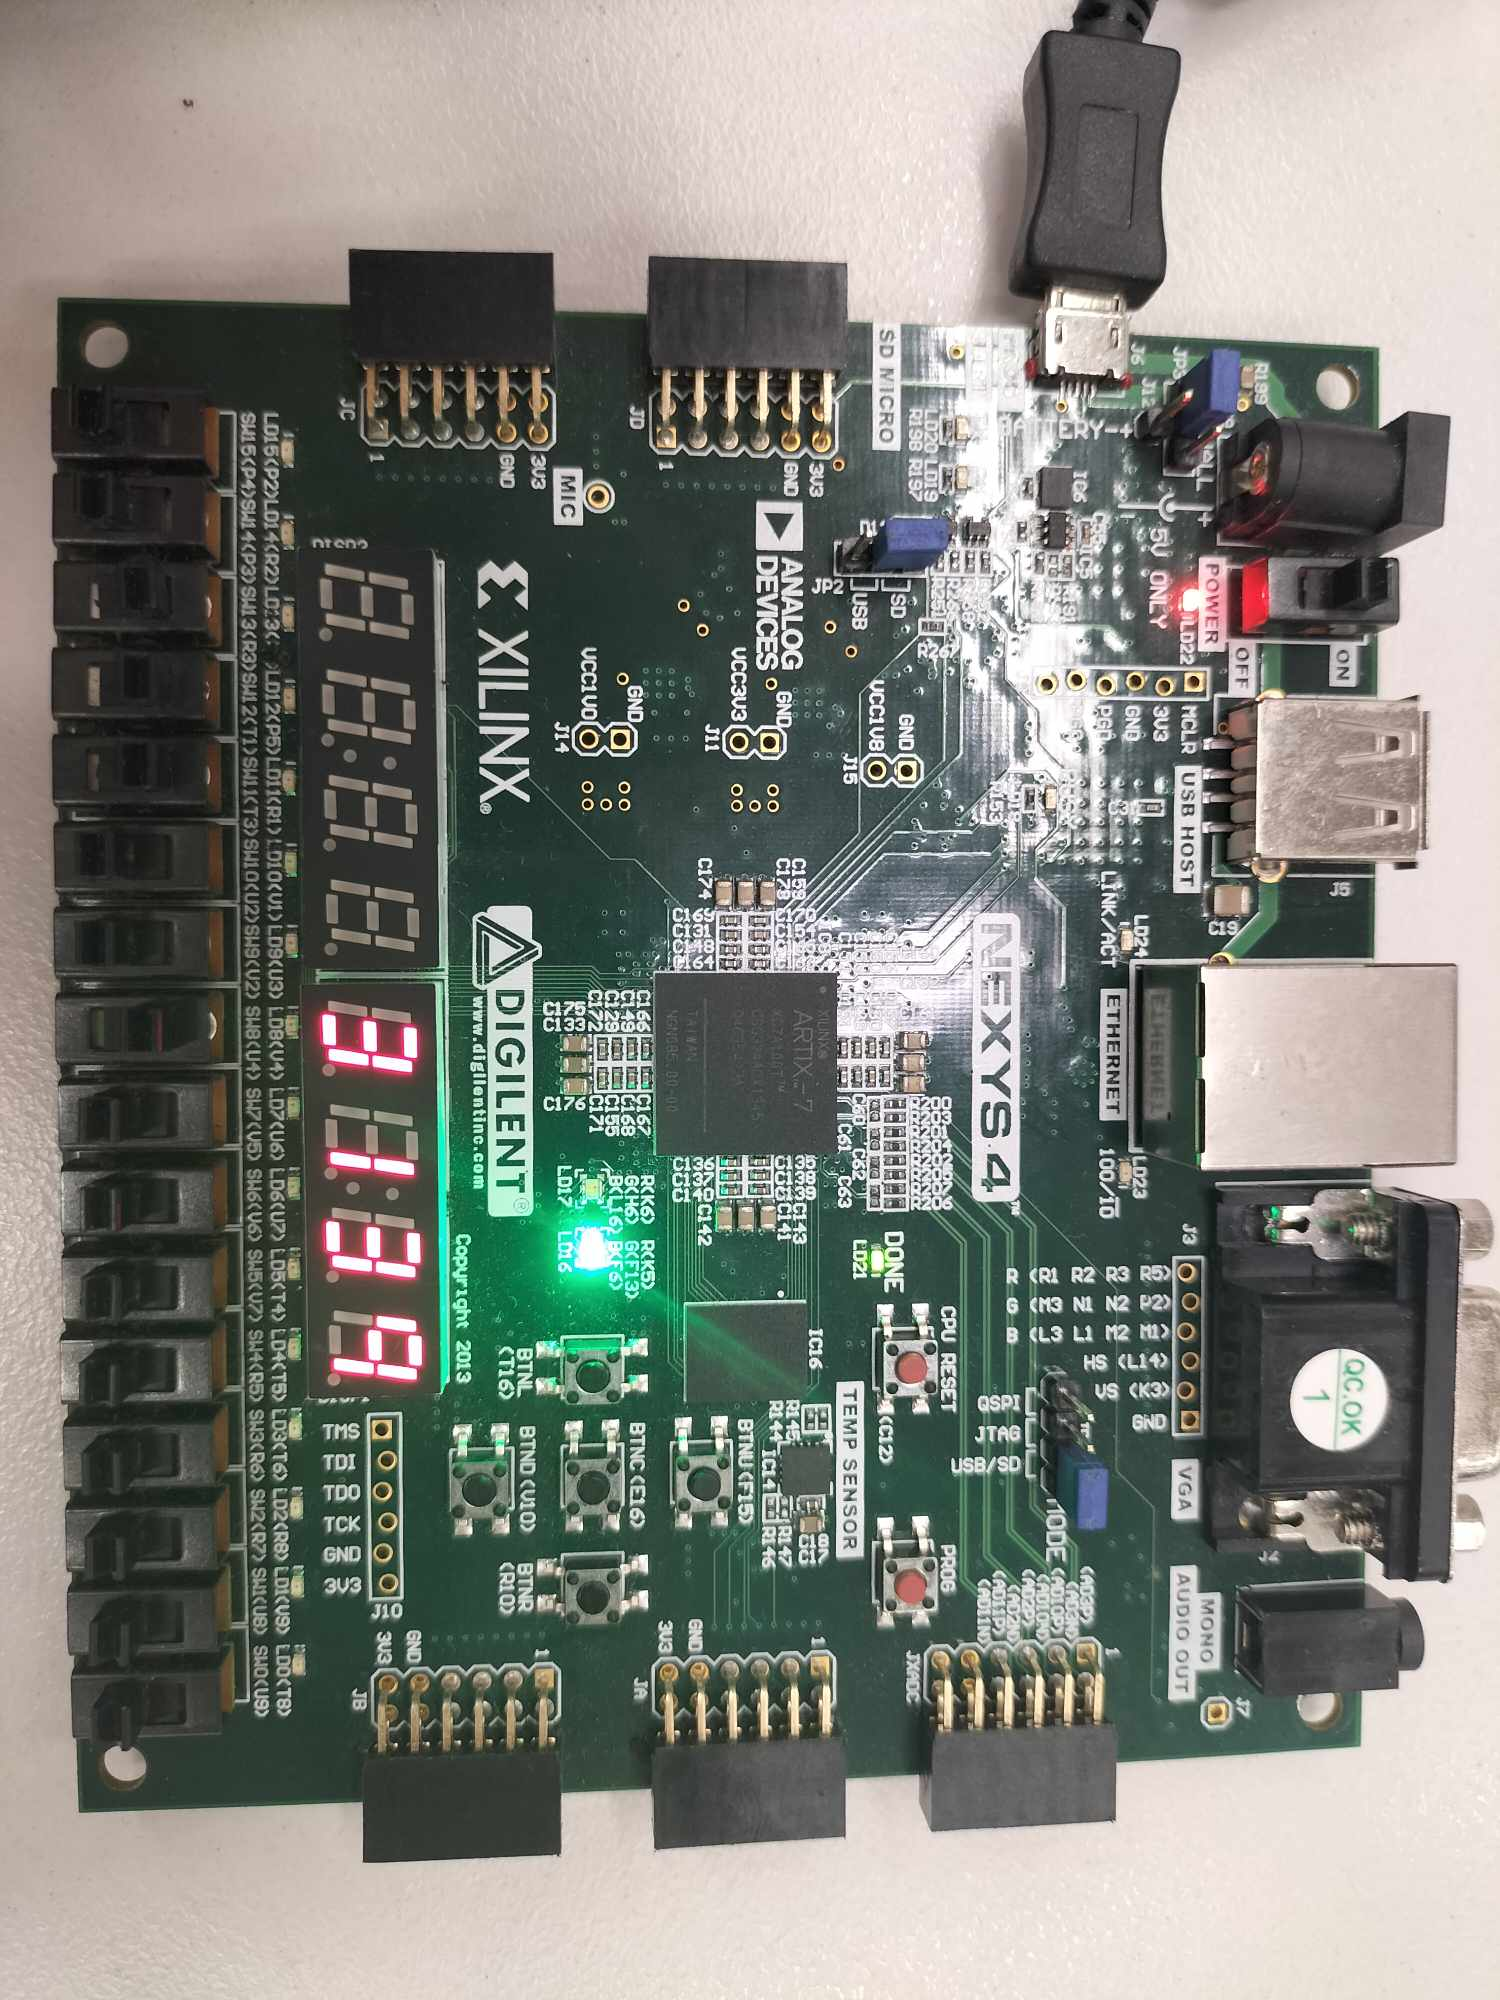
\includegraphics[scale=0.25]{images/fpga_2.jpg}
    \caption{FPGA with correct combination. Notice that the LED has switched from locked to unlocked state}
    \label{fig:fpga_2}
\end{figure}

\begin{figure}[H]
    \centering
    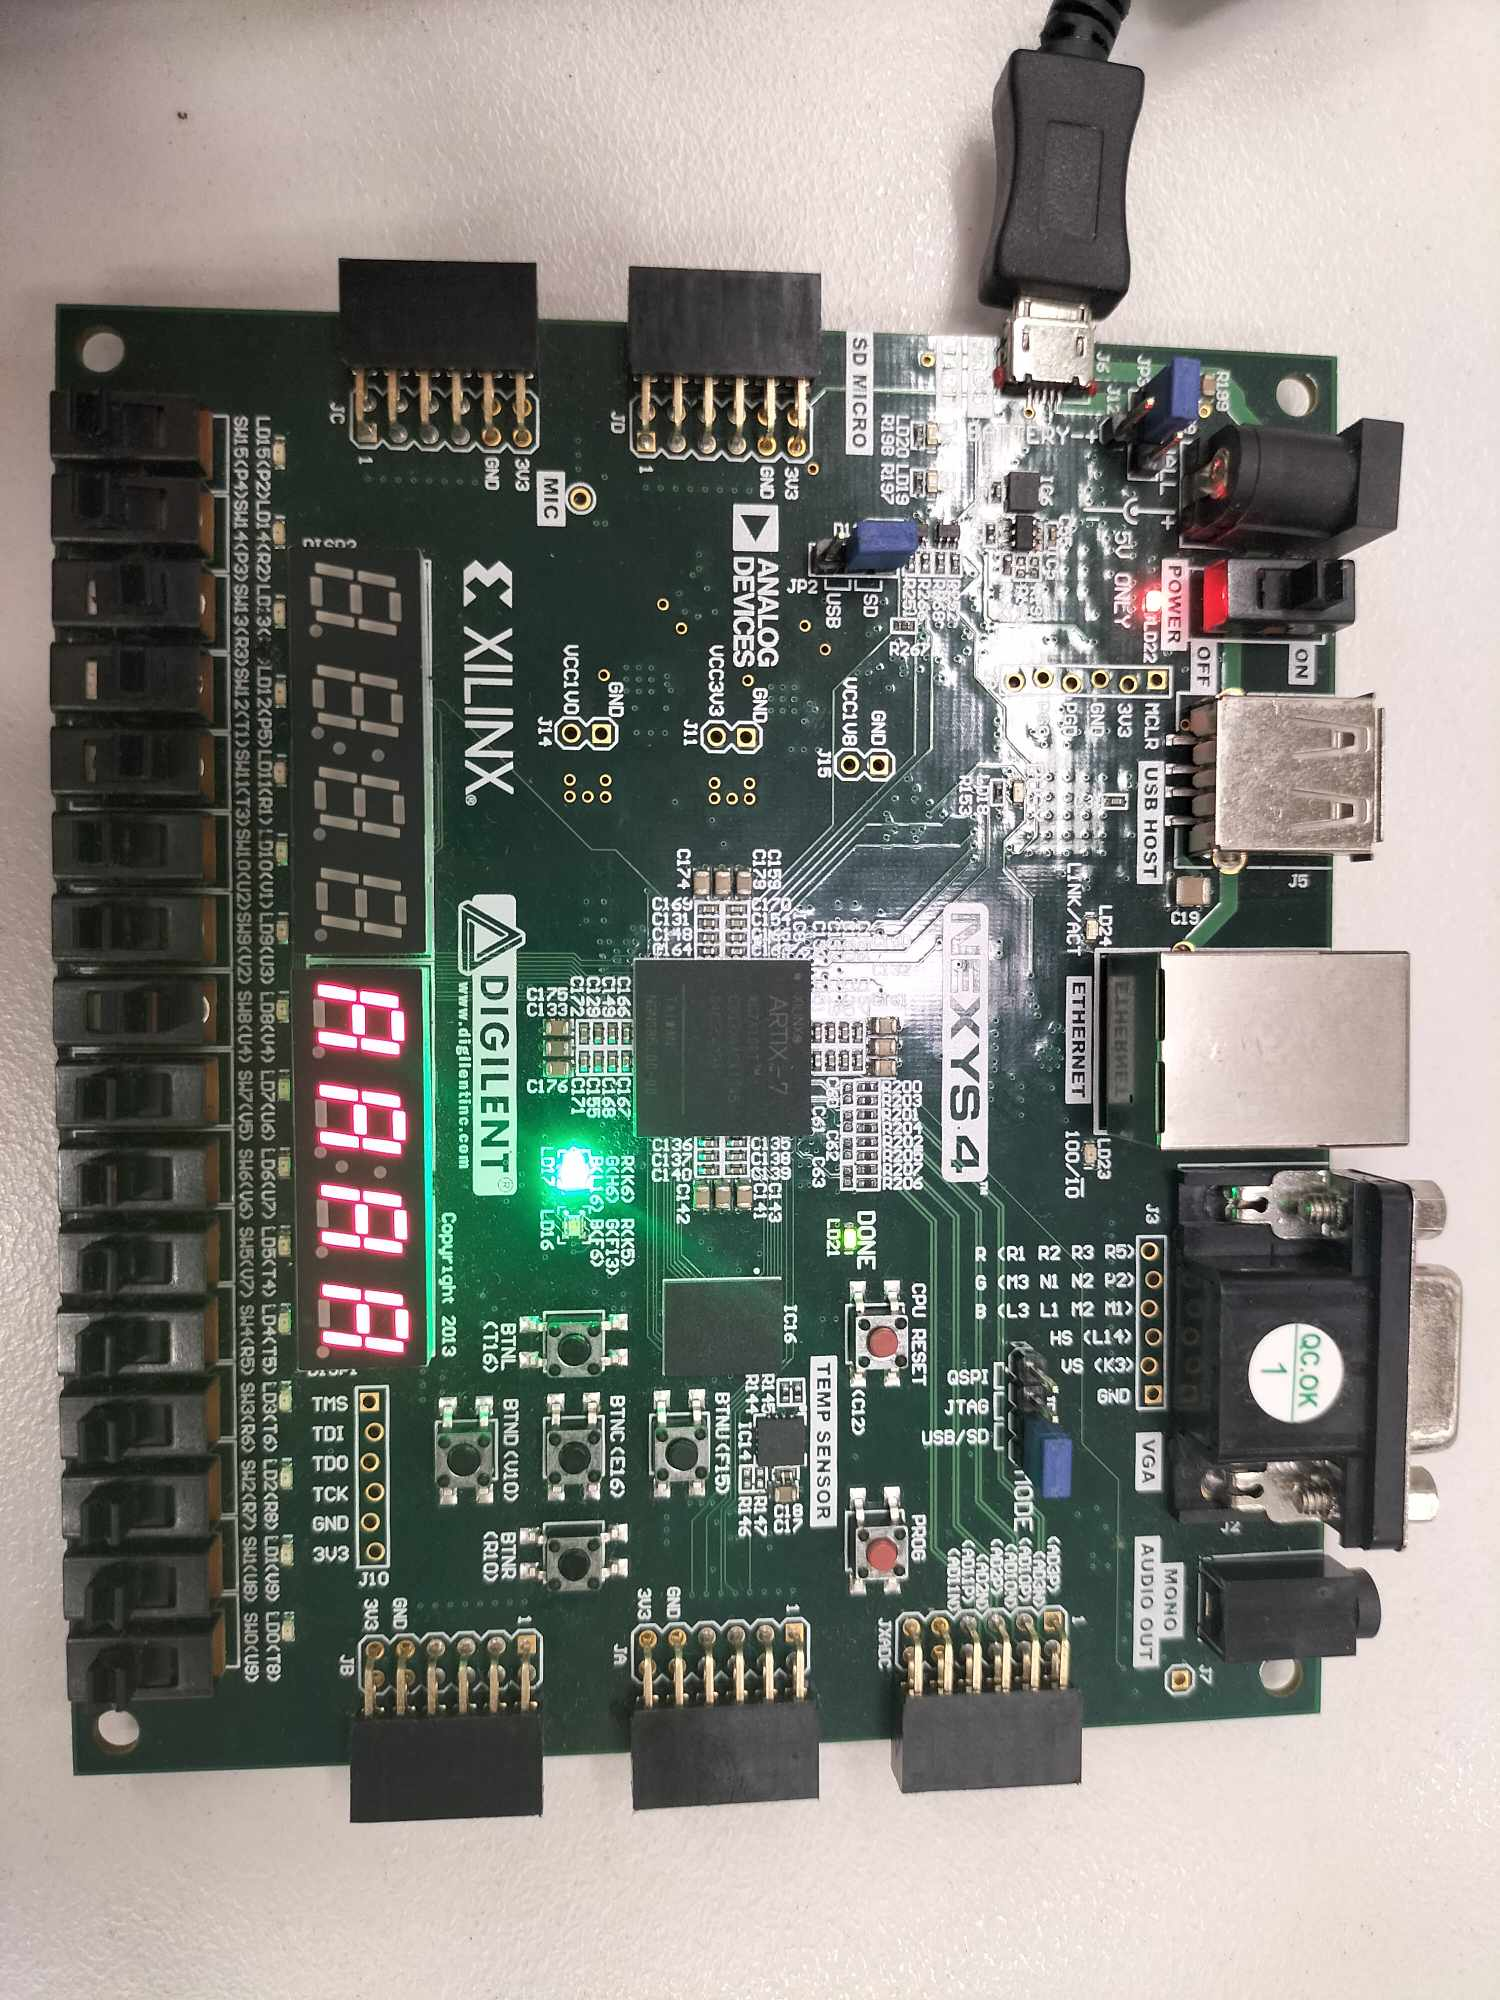
\includegraphics[scale=0.25]{images/fpga_reset.jpg}
    \caption{FPGA after selecting the reset switch}
    \label{fig:fpga_reset}
\end{figure}

As can be seen, total usability has been obtained and the system operates as per the design requirements.

\section{Register Transfer Level Schematic}

Figure \ref{fig:rtl} shows the top level design of the RTL schematic. This is going to be explained in greater detail in this segment.

\begin{figure}[H]
    \centering
    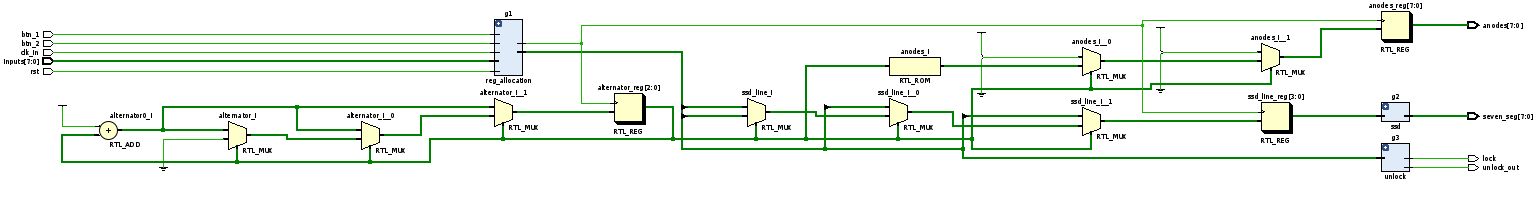
\includegraphics[scale=0.25]{images/rtl.png}
    \caption{Register Transfer Level top level view}
    \label{fig:rtl}
\end{figure}

Xilinx is a bit like fearless leader Ian Clough. It's been around alot longer than I have, and it knows how to optimize a circuit schematic far more efficiently. For this reason, the logic behind RTL designs often look different from the ones that are implemented in code; they do the same thing, just far faster. The areas in blue represent the subsystems for the locking mechanism, SSD and register allocation. Everything around them is simply multiplexers and look-up tables.

And that is an important distinction to make. On the implementation level, Xilinx does EVERYTHING with look-up tables. That's because the Nexys FPGAs are designed using LUTs, which can be seen upon close inspection of the design implementation. Everything else, such as the AND gates that will be seen later are abstract concepts that appear purely in the RTL.

In investigating the register allocation subsystem closely in figure \ref{fig:reg_all_close}, the multiplexing and LUT subsystems come into heavy play again. The presence of the buttons and clock as inputs requires the use of AND gates along with adders and subtractors to detect which button presses are present during the rising clock edges. The storing of the input values themselves are operated by the multiplexers connected to the LUT on the far right of the diagram.

\begin{figure}[H]
    \centering
    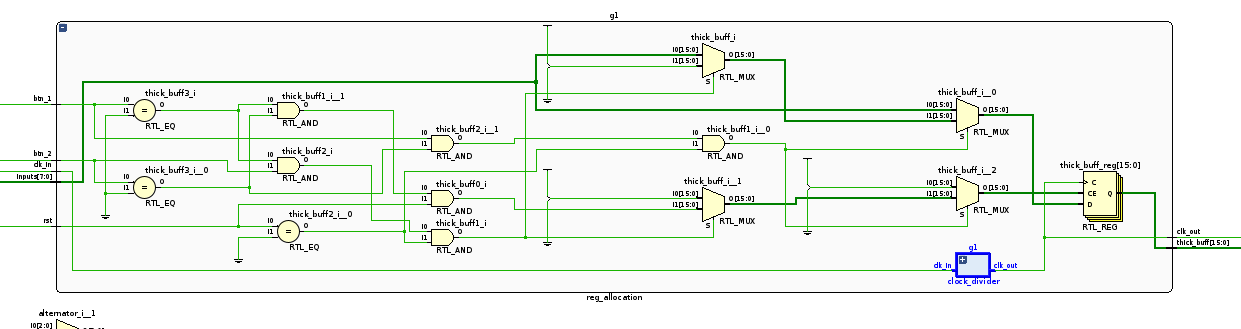
\includegraphics[scale=0.25]{images/reg_all_close.png}
    \caption{Register Transfer Level view of the register allocation subsystem}
    \label{fig:reg_all_close}
\end{figure}

The other subsystems in which data is stored are the locking and ssd mechanisms. These registers can also be found within figure \ref{fig:others_close}

\begin{figure}[H]
    \centering
    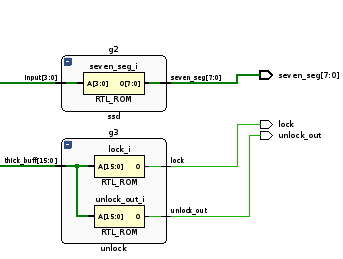
\includegraphics[scale=0.25]{images/others_close.png}
    \caption{Register Transfer Level view of the SSD and locking subsystems}
    \label{fig:others_close}
\end{figure}

\section{Synthesis Results}

There were several key features shown in the synthesis of the model. The first of these was the memory usage of the entire design. As can be seen in figure \ref{fig:memory}, less than $1\%$ of the entire system's memory was used, both in look-up tables and registers. The majority of memory usage came the the register-allocating system, which used 19 of the 26 LUTs and 31 of the 41 registers.

\begin{figure}[H]
    \centering
    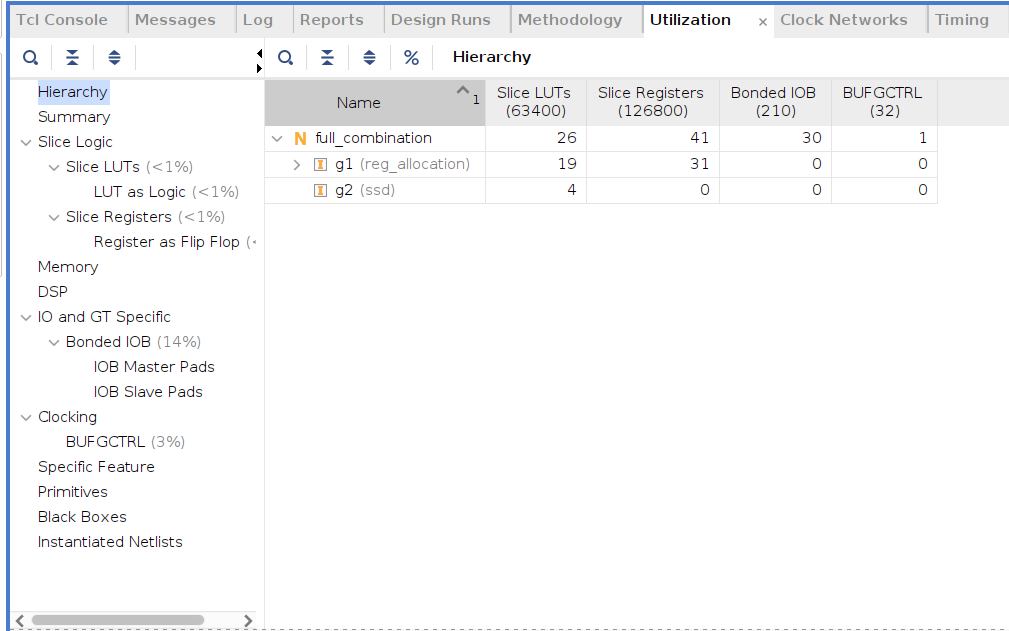
\includegraphics[scale=0.25]{images/memory_utilisation.png}
    \caption{Memory utilisation following synthesis}
    \label{fig:memory}
\end{figure}

In order to show the synchronicity of the system, it was also necessary to show the clock network. Figure \ref{fig:clk_network} displays the network of connections to the single 100MHz internal clock. Note that there are 27 variables that are not directly connected to the clock. These are internal signals, and were controlled via processes that were reliant upon the clock, thus maintaining system synchronicity. However, meshing the system to be completely connected to the 100MHz clock could be a suggested improvement, but it's not necessary for functionality.

\begin{figure}[H]
    \centering
    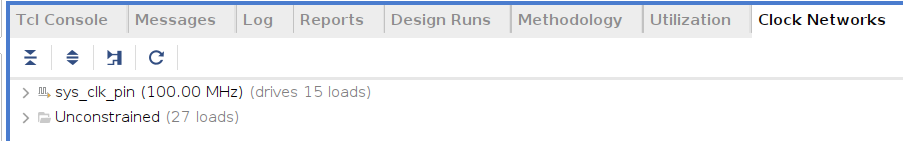
\includegraphics[scale=0.25]{images/clk_network.png}
    \caption{Synthesis showing the network of connections aligned with the 100MHz clock}
    \label{fig:clk_network}
\end{figure}

The other issue worth considering for synchronicity is the device's timing. Figure \ref{fig:timing} shows the synthesis results for timing, and indicates that there are no failings throughout the entire system. 

\begin{figure}[H]
    \centering
    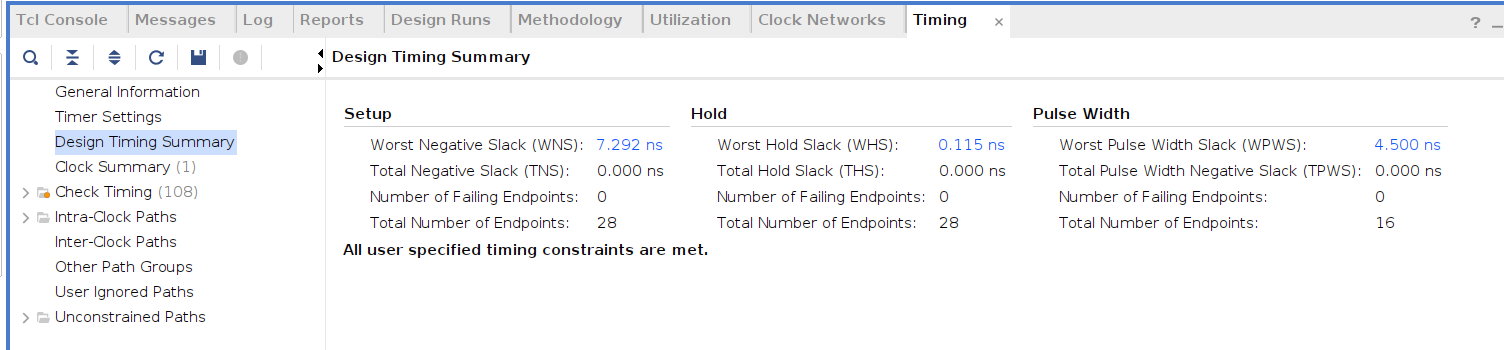
\includegraphics[scale=0.25]{images/synthesis_timing.png}
    \caption{Timing of the synthesis showing that there are no failings with timing during implementation}
    \label{fig:timing}
\end{figure}

\section{Conclusion}

In conclusion the system works as intended. The entire design criteria was satisfied. The system locks, unlocks and resets when prompted. Lastly, it does so in a synchronous fashion.

As a future improvement on the design, it could be possible to implement it in such a way that the 100MHz clock is able to connect to every signal in the program, thus eliminating any error warnings associated with it. As discussed in the synthesis section, however, this will not impact the usability of the design.

\end{document}
